\documentclass[tikz,border=10pt]{standalone}
\usepackage{tikz}
\usetikzlibrary{shapes, arrows.meta, positioning}

\begin{document}
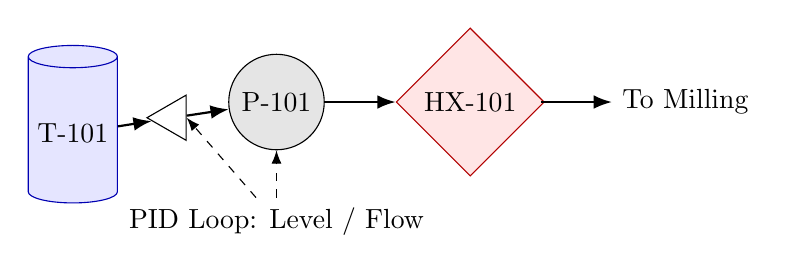
\begin{tikzpicture}[
  tank/.style={cylinder, draw=blue!70!black, aspect=0.25, shape border rotate=90, minimum height=2cm, minimum width=1cm, fill=blue!10},
  pump/.style={circle, draw=black, fill=gray!20, minimum size=0.8cm},
  hex/.style={diamond, draw=red!70!black, fill=red!10, minimum size=1cm},
  valve/.style={regular polygon, regular polygon sides=3, draw=black, fill=white, minimum size=0.4cm, rotate=90},
  arrow/.style={-Latex, thick}
]

\node[tank] (tank1) {T-101};
\node[valve, right=0.7cm of tank1] (valve1) {};
\node[pump, right=0.7cm of valve1] (pump1) {P-101};
\node[hex, right=0.9cm of pump1] (hx1) {HX-101};

\draw[arrow] (tank1) -- (valve1);
\draw[arrow] (valve1) -- (pump1);
\draw[arrow] (pump1) -- (hx1);
\draw[arrow] (hx1) ++(0.9,0) -- ++(0.9,0) node[right]{To Milling};

\node[below=0.6cm of pump1] (ctrl) {PID Loop: Level / Flow};
\draw[dashed, -Latex] (ctrl) -- (valve1.south);
\draw[dashed, -Latex] (ctrl) -- (pump1.south);

\end{tikzpicture}
\end{document}
